\chapter{Materials and methods}

\section{Datasets}

  Five datasets have been used in the framework of this thesis:
  one for training the model, one for optimizing the hyper-parameters, and three for benchmarking.
  The training set is a set of 354 proteins including the 150 families reported in the original PSICOV
  paper~\cite{doi:10.1093/bioinformatics/btr638}, plus a subset of the first benchmark set used by
  Michel et al. to evaluate PConsC3~\cite{Skwark079673}.
  The validation set is composed of the 30 protein families from the validation set of PConsC3,
  which itself is a subset of the test set of PConsC2~\cite{10.1371/journal.pcbi.1003889}.

  Three test sets have also been considered in order to make a direct comparison with the state-of-the-art RaptorX-Contact predictor.
  The first test set embodies the 105 protein domains from the CASP11 experiment, the second test set 76 proteins from the CAMEO
  project, and the fourth test set 398 membrane proteins.

  \subsection{Homology reduction}

    A straightforward method for reducing homology between two set of proteins is to
    remove proteins that have a sequence identity rate above a given threshold.
    As a rule of thumb, this threshold is usually set to 40\%.
    Identity rates were computed by running Needleman-Wunsch algorithm on each
    pair of proteins coming from two different datasets. Score matrix was set
    such that exact matches give a score of 1 and any mismatch gives a penalty of -1.
    Indeed this approach promotes global alignments with maximum identity rates.

    \begin{table}[H]
      \centering
      \begin{tabular}{|l|c|c|c|}
        \hline
        Identity rate & Minimum & Average & Maximum \\
        \hline
        \hline
        Training set - CASP11 & 5.4 & 22.4 & 32.5 \\
        PSICOV150 - CASP11 & 7.3 & 22.9 & 39.7 \\
        PSICOV150 - CAMEO & 6.2 & 21.7 & 34.4 \\
        Training set - CAMEO & 4.0 & 21.3 & 32.5 \\
        PSICOV150 - Membrane & 7.6 & 22.2 & 74.0 \\
        \hline
      \end{tabular}
      \captionof{table}{Identity rates between training and benchmark sets, expressed as percentages.}
      \label{identityrates}
    \end{table}

    Similarity rates are more informative than identity rates because amino acids
    are very likely to mutate across evolution towards amino acids that share
    similar physico-chemical properties, and such measures take these mutations
    into account. However, ECOD H-classes~\cite{10.1371/journal.pcbi.1003926}
    were used instead of similarity rates because they can potentially give more
    evidence on whether two sequences are evolutionary related.
    Therefore, proteins belonging to different datasets and sharing the same
    ECOD H-class have been rejected.

    \todo{Computation of identity rates, Common ECOD H-classes}

    \begin{figure}[H]
      \begin{center}
        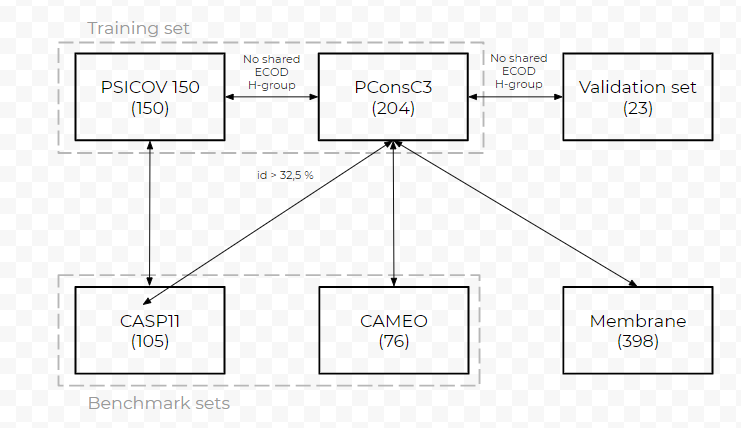
\includegraphics[width=\textwidth, keepaspectratio]{imgs/datasets.png}
         \caption{Homology reduction between the different datasets}
        \label{homology_reduction}
      \end{center}
    \end{figure}

  \subsection{PSICOV Dataset}

    The PSICOV~\cite{doi:10.1093/bioinformatics/btr638} dataset is composed of 150 families
    and associated multiple sequence alignments
    taken from the Pfam database, each containing more than 1000 homologous sequences
    and a target sequence with high-resolution ($\le$ 1.9 \AA{}) X-ray crystallographic structure.
    Each target sequence contains exactly one copy of the Pfam domain, has a length lower than
    275 and greater than 50 residues. The number of unique sequences in each multiple sequence
    alignment strongly varies from one family to another.
    AraC-like ligand binding domain (implied in DNA-binding transcription and
    sequence-specific DNA binding) accounts for 511 unique sequences, compared to 74 836 sequences
    for the response regulator receiver domain.

  \subsection{CASP11}

    CASP10~\cite{doi:10.1002/prot.24452}
    CASP11~\cite{doi:10.1002/prot.25064}


    \todo{}

  \subsection{CAMEO}

    CAMEO~\cite{haas2013protein}

    \todo{}

  \subsection{Membrane proteins}

    \todo{}

  \subsection{Feature extraction}

    \todo{Profile HMMs: \cite{eddy1998profile}}
    MSAs have been created using HHblits~\cite{HHblits} (version as of the date of 26th February 2016) on the Uniprot20 database
    with an e-value of 1. Parameters have been set in such a way that all sequences in each of the database MSAs are aligned.
    The obtained MSAs have been used as input to all other predictors and intermediate predictors, allowing for easier comparability.

    All protein sequences, structures, MSAs and intermediate predictions used in this thesis come from the datasets that were publicly
    available at the address \url{http://pconsc3.bioinfo.se/pred/download/} as on the date of 28th December 2018.
    Information available in these datasets is the following:

    \todo{PDB parser to obtain distance and contact maps}

    \begin{itemize}
      \item Protein sequence in FASTA format
      \item \index{MSA} obtained using HHblits on the corresponding protein family
      \item Atom 3D coordinates
      \item PhyCMAP~\cite{PhyCMap} intermediate predictions
      \item plmDCA~\cite{EKEBERG2014341} intermediate predictions
      \item GaussDCA~\cite{10.1371/journal.pone.0092721} intermediate predictions
      \item Predictions made by PConsC3~\cite{Skwark079673} at each layer of the model
      \item CCMPred~\cite{CCMPred} predictions (only available in the 4 test sets)
      \item EVFold~\cite{Sheridan021022} predictions (only available in the 4 test sets)
      \item PSICOV~\cite{doi:10.1093/bioinformatics/btr638} predictions (only available in the 4 test sets)
      \item MetaPSICOV~\cite{MetaPSICOV} predictions (only available in the 4 test sets)
    \end{itemize}

    \todo{Took alignments from PConsC2 and PConsC3 -> model not influenced by the new releases of alignments tools}
    \todo{What about the protein structures?}

    \todo{Oversampling negative class: \cite{markowski2016oversampling}}